\documentclass[aspectratio=169,11pt]{beamer}
\usepackage{teaching_slides}


\title[L4 - Inference and Standard Errors]{ Econometrics I}
\subtitle{Lecture 3a: Inference and Standard Errors}
\author{Chris Conlon}
\date{Fall 2026}


\begin{document}
\maketitle




\begin{frame}
\begin{center}
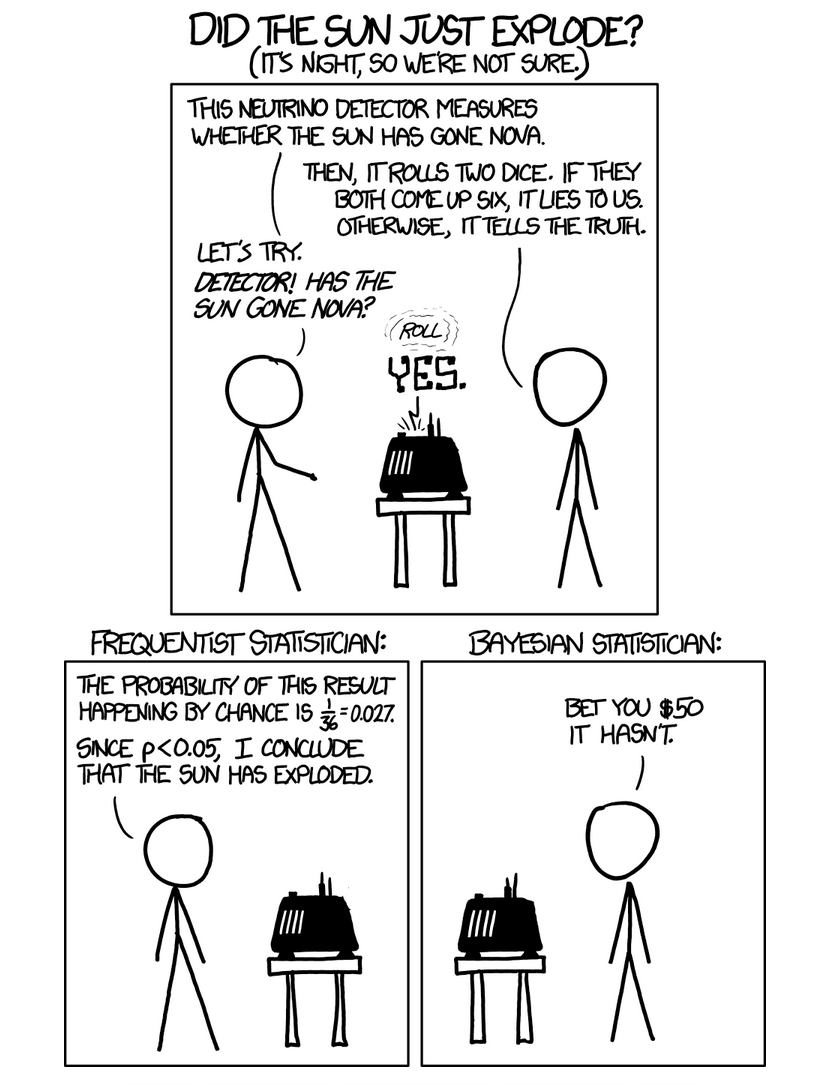
\includegraphics[height=.92\textheight]{explode} \\
{\tiny Source: xkcd.com}
\end{center}
\end{frame}


\begin{frame}{Before the formulas: what are we uncertain about?}
\begin{itemize}
	\item Every inference question starts with an \alert{estimand}: the number you
	would compute with infinite data. An elasticity. A treatment effect. The
	gender gap in log wages. (Goff's Appendix C calls this
	``defining the parameter of interest,'' and puts it \emph{before} estimation.)

	\medskip
	\item A standard error quantifies exactly one kind of uncertainty:
	\alert{sampling uncertainty} --- you have $n$ observations instead of all of them.

	\medskip
	\item It says \emph{nothing} about the other ways to be wrong:
	omitted variables (last week), measurement error, the wrong functional form,
	the wrong estimand.

	\medskip
	\item Corollary you already simulated: the short regression in the Silly Example
	has a \alert{tiny standard error around the wrong number}. Precision is not
	validity.
\end{itemize}
\medskip
Today: how to get the sampling uncertainty right. Keep asking the other questions anyway.
\end{frame}



\section{Recap: Asymptotics for OLS and the Linear Model}


\begin{frame}{OLS}
\begin{align*}
y_i = \beta_0 + \beta_1 x_i + \varepsilon_i
\end{align*}
Recall the three basic OLS assumptions
\begin{enumerate}
\item $\E\left[\varepsilon_i |x_i \right] = 0$
\item $(x_i,y_i)$, $i =1,\ldots,n$, are i.i.d.
\item Large outliers are rare: $\E\left[y_i^4\right]< \infty$ and $\E\left[x_i^4\right]<\infty$.
\end{enumerate}
\end{frame}

\begin{frame}{Unbiasedness and Consistency}
\begin{itemize}
\item Unbiasedness means that, on average, an estimator $\widehat{\theta}$ neither over- nor under-estimates the true $\theta$:
\begin{align*}
\E[\widehat{\theta} ] - \theta = 0
\end{align*}
\item Consistency tells us that we approach the true $\theta$ as $n \rightarrow \infty$.
\begin{align*}
\widehat{\theta}  \overset{p}{\to} \theta
\end{align*}
\item Example: $X_{1}$ (the first observation) is unbiased but not consistent for the mean.
\item Example: $\frac{n}{n-5} \overline{X}$ is consistent but biased for the mean.
\end{itemize}
\end{frame}



\begin{frame}{Outliers}
\begin{itemize}
	\item {\bf Outliers} refer to observations that are ``far away'' from the rest of the data. 
	They can be due to errors in the data.  There is no standard formal definition. 

	\medskip
	\item What to do? Greene:``\emph{It is difficult to draw firm general conclusions... It remains likely that in very
	small samples, some caution and close scrutiny of the data are called for.}'' I'd say that's true even in large samples,
	but there isn't a generally accepted way of quantifying what counts as appropriate ``caution and close scrutiny.''


\end{itemize}
\end{frame}


\begin{frame}{Removing Outliers?}
\begin{itemize}
\item Removing extreme outliers (in $x$) from datasets is often considered good practice. But we should be mindful
		about why as dropping observations creates the potential for manipulation. 

	\medskip
	\item Sometimes extreme outliers are just errors, in which case they should almost certainly be dropped.

	\medskip
	\item Even if they aren't errors, they may reflect a different mode in the data generating process. They may require
		a different or more general model to account for them properly. Consider the justification of a linear
		model based on Taylor's theorem (local linear approximation). With such a justification for your modeling
		strategy, it would not make sense to include an outlier in $x$.
	\medskip
	\item It's important to be transparent about how dropped outliers affect results. 

\end{itemize}
\end{frame}




\begin{frame}{Outliers and Leverage}
\begin{itemize}
\item One way to find influential observations is to calculate the {\bf leverage} of each observation $i$. We begin with the hat matrix:
\begin{align*}
{\bf P} = {\bf X} ({\bf X} '{\bf X})^{-1}  {\bf X}'
\end{align*}
and consider the diagonal elements, which are labeled $h_{ii}$
\begin{align*}
h_{ii} = {\bf x}_i' ({\bf X} '{\bf X})^{-1}  {\bf x}_i
\end{align*}

\medskip
\item This tells us how influential an observation is in our estimate of ${\bf b}_{OLS}$.\\
Particularly important for $\{0,1\}$ dummy variables with uneven groups.
\end{itemize}
\end{frame}



\begin{frame}{Leave One Out Regression}
\begin{itemize}
\item This is sometimes called the {\bf Jackknife}
\item Sometimes it is helpful to know what would happen if we omitted a single observation $i$
\item Turns out we don't need to run $n$ regressions
\begin{align*}
{\bf b}_{-i} &= ({\bf X}_{-i}'{\bf X}_{-i})^{-1} {\bf X}_{-i}' {\bf y}_{-i} \\
&={\bf b}_{OLS} -  ({\bf X} '{\bf X})^{-1} {\bf x}_i  \tilde{e}_i  \quad \mbox{ where } \tilde{e}_i = (1-h_{ii})^{-1} e_i
\end{align*}
\item $\tilde{e}_i $ has the interpretation of the LOO prediction error.
\item high leverage observations move ${\bf b}_{OLS}$ a lot.
\end{itemize}
\end{frame}


% \begin{frame}{Outliers and Leverage}
% One way to find \alert{outliers} is to calculate the \alert{leverage} of each observation $i$. We begin with the \alert{hat matrix}:
% \begin{align*}
% P = X  (X'X)^{-1} X'
% \end{align*}
% and consider the diagonal elements which for some reason are labeled $h_{ii}$
% \begin{align*}
% h_{ii} = x_i (X'X)^{-1} x_i'
% \end{align*}
% This tells us how \alert{influential} an observation is in our estimate of $\widehat{\beta}$.\\
% Particularly important for $\{0,1\}$ \alert{dummy variables} with uneven groups.
% \end{frame}


% \begin{frame}{Leave One Out Regression}
% \begin{itemize}
% \item This is sometimes called the \alert{Jackknife}
% \item Sometimes it is helpful to know what would happen if we omitted a single observation $i$
% \item Turns out we don't need to run $N$ regressions
% \begin{align*}
% \widehat{\beta}_{-i} &= (X_{-i}'X_{-i})^{-1} X_{-i}' Y_{-i} \\
% &=\widehat{\beta} -  (X 'X)^{-1} x_i  \tilde{u}_i  \quad \mbox{ where } \tilde{u}_i = (1-h_{ii})^{-1}\hat{u}_i
% \end{align*}
% \item $\tilde{u}_i $ has the interpretation of the \alert{LOO prediction error}.
% \item high leverage observations move $\widehat{\beta}$ a lot.
% \end{itemize}
% You can read more about this in Ch3 of Hansen. [Skip derivation]
% \end{frame}

% Bias-variance decomposition moved to L2 (estimator MSE, with a shrinkage simulation), Fall 2026.
\begin{frame}{Variance of ${\bf b}_{OLS}$}
\begin{itemize}
	\item A useful identity for linear algebra (scalar $a$, fixed matrix ${\bf A}$, random vector ${\bf z}$):
\begin{align*}
\Var (a {\bf z} ) &= a^2 \Var({\bf z})\\
\Var ({\bf A} {\bf z} ) &= {\bf A}  \Var({\bf z}) {\bf A}'
\end{align*}

\smallskip
\item Since ${\bf b}_{OLS} = ({\bf X}' {\bf X} )^{-1} {\bf X}' {\bf y}$,
\begin{align*}
\Var ({\bf b}_{OLS} \mid  {\bf X}) = ({\bf X}' {\bf X} )^{-1} \, {\bf X}' \, \Var ({\bf y} \mid {\bf X}) \,  {\bf X} \, ({\bf X}'{\bf X} )^{-1}
\end{align*}

\smallskip
\item Recalling that $\Var ( {\bf y} \mid {\bf X} )  = \Var ( \boldsymbol{\varepsilon}  \mid {\bf X}  ) $ (because ${\bf X}\boldsymbol{\beta}$ is fixed given ${\bf X}$),
\begin{align*}
\Var( {\bf b}_{OLS} \mid {\bf X}) = ({\bf X}'{\bf X})^{-1}\, {\bf X}'\, \Var ( \boldsymbol{\varepsilon} \mid {\bf X} ) \, {\bf X} \, ({\bf X}'{\bf X})^{-1}
\end{align*}
\end{itemize}
\end{frame}




\begin{frame}{Variance of ${\bf b}_{OLS}$}
Start with the variance of the errors to form a \alert{diagonal} matrix ${\bf D}$:
\begin{align*}
\Var ( \boldsymbol{\varepsilon} | {\bf X} ) &= \E \left[ \boldsymbol{\varepsilon} \boldsymbol{\varepsilon}' \mid {\bf X} \right] = {\bf D}\\
{\bf D} &= \operatorname { diag } \left( \sigma _ { 1 } ^ { 2 } , \ldots , \sigma _ { n } ^ { 2 } \right) = \left( \begin{array} { c c c c } { \sigma _ { 1 } ^ { 2 } } & { 0 } & { \cdots } & { 0 } \\ { 0 } & { \sigma _ { 2 } ^ { 2 } } & { \cdots } & { 0 } \\ { \vdots } & { \vdots } & { \ddots } & { \vdots } \\ { 0 } & { 0 } & { \cdots } & { \sigma _ { n } ^ { 2 } } \end{array} \right)
\end{align*}
\begin{itemize}
\item ${\bf D}$ is diagonal because, for $i \ne j$, $\E[\varepsilon_i \varepsilon_j \mid  {\bf X}] = \E[\varepsilon_i  \mid {\bf x}_i] \cdot \E[\varepsilon_j  \mid  {\bf x}_j]=0$ (independence across observations)
\item The diagonal elements of ${\bf D}$ are $\E[\varepsilon_i^2 \mid  {\bf X}] = \E[\varepsilon_i^2 \mid {\bf x}_i] = \sigma_i^2$.
\item In the \alert{homoskedastic} case ${\bf D} = \sigma^2 {\bf I}_n$.
\end{itemize}
\end{frame}


\begin{frame}{Variance of ${\bf b}_{OLS}$}
\small
Let $\widetilde{{\bf D}} = \operatorname{diag}\left(\varepsilon_1^2,\ldots,\varepsilon_n^2\right)$. Then
\begin{align*}
{\bf D} = \operatorname { diag } \left( \sigma _ { 1 } ^ { 2 } , \ldots , \sigma _ { n } ^ { 2 } \right)
= \E \left[ \widetilde{{\bf D}} \mid  {\bf X} \right]
\end{align*}

An (infeasible, since $\boldsymbol{\varepsilon}$ is unobserved) estimator of ${\bf V}_{{\bf b}} = \Var({\bf b}_{OLS}|{\bf X})$ plugs in $\widetilde{{\bf D}}$ for ${\bf D}$:
\begin{align*}
\widehat{{\bf V}}_{{\bf b}}^{\text{ideal}} &= ({\bf X}'{\bf X})^{-1} ({\bf X}'  \widetilde{{\bf D}} {\bf X}) ({\bf X}'{\bf X})^{-1}
= ({\bf X}'{\bf X})^{-1} \left(\sum_{i=1}^n {\bf x}_i {\bf x}_i' \varepsilon_i^2  \right) ({\bf X}'{\bf X})^{-1} 
\end{align*}
The expectation shows us this estimator is unbiased:
\begin{align*}
\E[\widehat{{\bf V}}_{{\bf b}}^{\text{ideal}} \mid {\bf X}] &= ({\bf X}'{\bf X})^{-1} \left(\sum_{i=1}^n {\bf x}_i {\bf x}_i'\, \E[\varepsilon_i^2 | {\bf X}] \right) ({\bf X}'{\bf X})^{-1} \\
&= ({\bf X}'{\bf X})^{-1} \left(\sum_{i=1}^n {\bf x}_i {\bf x}_i' \, \sigma_i^2 \right) ({\bf X}'{\bf X})^{-1} = ({\bf X}'{\bf X})^{-1} ({\bf X}' {\bf D} {\bf X}) ({\bf X}'{\bf X})^{-1} = {\bf V}_{{\bf b}}
\end{align*}
\end{frame}




\begin{frame}{Heteroskedasticity Consistent (HC) Variance Estimates}
Replace the unobserved $\varepsilon^2_i$ with squared OLS residuals $e_i^2$:
\begin{align*}
\widehat{{\bf V}}_{{\bf b}}^{HC0}&= ({\bf X}'{\bf X})^{-1} \left(\sum_{i=1}^n {\bf x}_i {\bf x}_i' e_i^2 \right) ({\bf X}'{\bf X})^{-1} \\
\widehat{{\bf V}}_{{\bf b}}^{HC1}&= ({\bf X}'{\bf X})^{-1} \left(\sum_{i=1}^n {\bf x}_i {\bf x}_i' e_i^2 \right) ({\bf X}'{\bf X})^{-1} \cdot \left(\frac{n}{n-K}  \right)
\end{align*}
Could use leave-one-out residuals $\tilde{e}_i = (1-h_{ii})^{-1}e_i$:
\begin{align*}
\widehat{{\bf V}}_{{\bf b}}^{HC2}&= ({\bf X}'{\bf X})^{-1} \left(\sum_{i=1}^n (1-h_{ii})^{-1} {\bf x}_i {\bf x}_i' e_i^2 \right) ({\bf X}'{\bf X})^{-1} \\
\widehat{{\bf V}}_{{\bf b}}^{HC3}&= ({\bf X}'{\bf X})^{-1} \left(\sum_{i=1}^n (1-h_{ii})^{-2} {\bf x}_i {\bf x}_i' e_i^2 \right) ({\bf X}'{\bf X})^{-1}
\end{align*}
\end{frame}

\begin{frame}{Heteroskedasticity Consistent (HC) Variance Estimates}
\begin{itemize}
\item We know that $\widehat{{\bf V}}_{{\bf b}}^{HC3} \ge \widehat{{\bf V}}_{{\bf b}}^{HC2} \ge \widehat{{\bf V}}_{{\bf b}}^{HC0}$ (in the positive-semidefinite sense) because $0 < 1- h_{ii} \le 1$.
\item $HC3$ are the most \alert{conservative} and also place the most weight on high-leverage observations.
\item \texttt{Stata} uses $HC1$ as the default and it is what most people refer to when they say \alert{robust standard errors}.
\item These are often called White (1980) SE's or Eicker-Huber-White SE's.
\item In small samples there is some evidence that $HC2$ has better \alert{coverage} (what is that?)
\end{itemize}
\end{frame}




\begin{frame}{Example: Engel Curves}
\begin{itemize}
	\item Engel curves refer to the relationship between a household's expenditure share on a 
	good and income (or total expenditure).

	\item Engel curves for food are typically downward sloping -- as total expenditure of a household
	increases, the proportion of its expenditure dedicated to food falls.
	\begin{itemize}
		\item Expenditure on food still rises as total expenditure rises, but less than proportionally,
		so that food's expenditure \emph{share} falls.
	\end{itemize}
\end{itemize}
\end{frame}




\begin{frame}{Food Engel Curves}
\begin{columns}
\begin{column}{0.5\textwidth}
	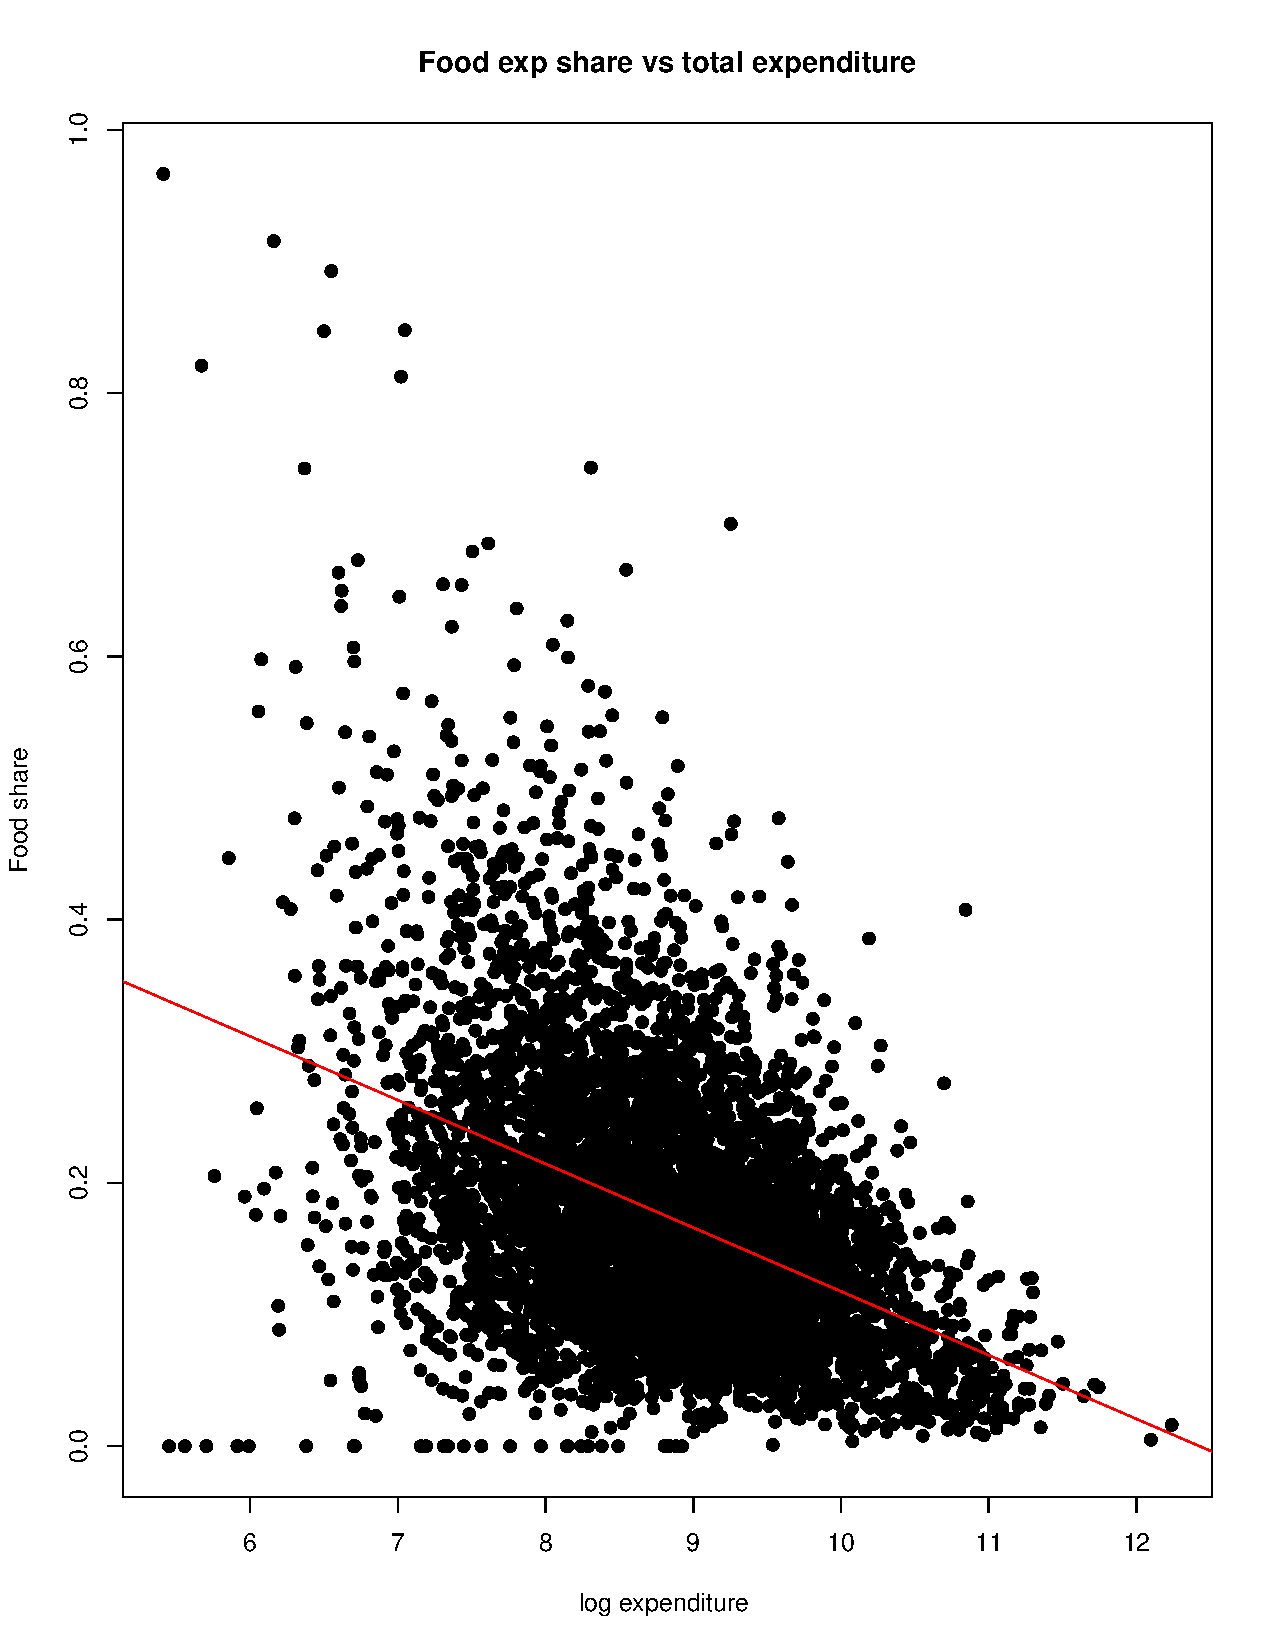
\includegraphics[width=.7\textwidth]{engle1.pdf}	

{\tiny Data source: BLS Consumer Expenditure Survey data}

\end{column}
\begin{column}{0.5\textwidth}
\begin{itemize}
	\item If we plotted total food expenditure (rather than the expenditure share), the heteroscedasticity would go in the other direction.
\end{itemize}
\end{column}
\end{columns}
\end{frame}



\begin{frame}{Heteroscedasticity vs. Correlation}
\begin{itemize}
	\item Recall that we defined the homoscedasticity assumption as:\[
	\Var\left(\boldsymbol{\varepsilon} | {\bf X}\right) =\sigma^2 {\bf I}
	\]
	this assumption has two aspects:
	\begin{enumerate}
		\item The disturbance for each observation has the same variance
		\item Imposing zero correlation between disturbances for different observations
	\end{enumerate}

	\item The terminology can be misleading here, because what people refer to as ``heteroscedasticity-robust''
	standard errors (the HC0--HC3 estimators above) are robust to violations of 1 but not 2. 

	\item We need to do a bit more to estimate standard errors in a way that is robust to correlated data. 

\end{itemize}
\end{frame}


\begin{frame}{Correlation I}
\begin{itemize}
	\item The baseline assumptions of the linear regression framework imply that
	the disturbances are uncorrelated across observations.  There are many ways for this to be violated. 
	\begin{itemize}
		\item Example 1: we might have county-level data for a regression and be concerned
		that different counties within a given state have correlated disturbances because
		all counties are subject to the same (unobserved) state-level policies.
		\item Example 2: time series data (asset prices), and we are worried that some unobserved
		factors within the disturbances are serially correlated
		\item Example 3: county level data again, and we are worried about geographically
		correlated factors such as weather. 
	\end{itemize}
\end{itemize}
\end{frame}


\begin{frame}{Correlation II}
 Different correlation patterns call for different estimators of ${\bf V}_{{\bf b}} = \Var\left({\bf b}_{OLS}|{\bf X}\right)$.
	Some common alternatives to the no-correlation baseline:
\begin{enumerate}
	\item Clustered standard errors, when there is correlation between observations
	within well-defined groups, but no correlation between observations in different groups. 
	\item Newey-West standard errors (and extensions) to deal with serial correlation
	in time series data.
	\item Conley-Newey-West standard errors that allow for correlation in multiple dimensions
	(especially popular in the context of spatially explicit models).
\end{enumerate}
\end{frame}


\begin{frame}{What is Clustering?}
Suppose we want to relax our i.i.d. assumption:
\begin{itemize}
\item Each observation $i$ is a \alert{villager} and each group $g$ is a \alert{village}
\item Each observation $i$ is a \alert{student} and each group $g$ is a \alert{class}.
\item Each observation $t$ is a \alert{year} and each entity $i$ is a \alert{state}.
\item Each observation $t$ is a \alert{week} and each entity $i$ is a \alert{shopper}.
\end{itemize}
We might expect that $\Cov (\varepsilon_{ig},\varepsilon_{jg}) \neq 0$ for $i \ne j$ in the same group $g$ $\rightarrow$ independence is a bad assumption. 
\end{frame}

\begin{frame}{Clustering: Intuition}
The groups (villages, classrooms, states) are independent of one another, but within each group we can allow for arbitrary correlation.
\begin{itemize}
\item If correlation is within an individual over time we call it \alert{serial correlation} or \alert{autocorrelation}
\item Just like in time-series$\rightarrow$ we have fewer effective independent observations in our sample.
\item Asymptotics now about the number of groups $G \rightarrow \infty$ not observations $n \rightarrow \infty$
\end{itemize}
\end{frame}


\begin{frame}{Clustering I}
\begin{itemize}
	\item Suppose data are organized into distinct groups $g=1,2,\dots,G$. Let $g\left(i\right)$
	be the group identity of observation $i$. 
	\begin{itemize}
		\item e.g., with county-level data, we have $g\left(\text{Manhattan}\right)=\text{NY}$.
	\end{itemize}


	\medskip
	\item We assume $\E\left[\varepsilon_i \varepsilon_j | {\bf X}\right]=0$ as long as $g\left(i\right)\ne g\left(j\right)$,
	and we do not restrict the correlation $\E\left[\varepsilon_i \varepsilon_j | {\bf X}\right]$
	for observations within the same group.

	\medskip
	\item Intuition: the linear regression framework with no correlation in observations will overstate
	the precision of our estimates. If we add another observation within a cluster, and that observation
	is highly correlated with the other observations, it's not actually as good as adding another independent observation. 
\end{itemize}
\end{frame}

\begin{frame}{Clustering II}
\begin{itemize}
	\item Recall the sandwich formula for standard errors:
		\begin{align*}
		\Var\left({\bf b}_{OLS}\right) \approx	n^{-1} \E\left[{\bf x}_i {\bf x}_i' \right]^{-1} \Var \left[{\bf x}_i \varepsilon_i \right] \E\left[{\bf x}_i {\bf x}_i' \right]^{-1}.
		\end{align*}

		% \item The estimator for the middle part without clustering was
		\begin{align*}
		\widehat{\Var}\left[{\bf x}_i \varepsilon_i \right] = n^{-1} \sum_{i} {\bf x}_i {\bf x}_i'  e_i^2
		\end{align*}

	% \item With clustering, it will be \[
	% {\symbf V}_{clu} = n^{-1} \sum_{i=1}^{n}\sum_{j=1}^{n} {\symbf x}_i\,  {\symbf x}'_j \, e_i\, e_j \cdot {\mathbb{I}}\left[(i,j) \in \text{Group}_g \right]
	% \]
	% where the ${\symbf I}$ function is 1 when $i,j$ come from the same group and zero otherwise.

\end{itemize}
\end{frame}



\begin{frame}{Clustering III}
\begin{itemize}
	\item The cluster-robust estimate of standard errors will be consistent as the number of groups 
	gets large.

	\item Note that this estimator adds extra terms (covariance terms) to the estimate of variance,
	so this is going to make standard errors larger as long as covariances $\E\left[\varepsilon_i \varepsilon_j\right]$ are positive. 

	\item Thus, if standard formulas are used in the presence of cluster-correlated disturbances, 
	standard errors will be too small.

	\item Statistical software packages typically make it easy to compute cluster-robust errors.
	
	\item Clustering often makes a {\bf huge} difference in standard errors.

\end{itemize}
\end{frame}

% \begin{frame}{Correlation III}

%  Consider the cluster-robust estimator of the ``meat'' part of the sandwich estimator: \[
% 	{\bf V}_{clu} = n^{-1} \sum_{i=1}^{n}\sum_{j=1}^{n} {\bf x}_i \, {\bf x}'_j \,  e_i \, e_j\, {\mathbb{I}}\left[g\left(i\right)==g\left(j\right)\right]
% 	\]

% \medskip
%  For Conley-Newey-West standard errors (where there is correlation between ``nearby'' observations),
% 	procedure is similar.

% \medskip
% 	 The difference is that instead of the 1/0 indicator function for ${\bf I}$, we will have a 
% 	weighting (or kernel) function which takes on values $\approx 1$ for ``nearby'' observations and goes to zero for
% 	observations that are far apart.


% \end{frame}


\begin{frame}{Clustering Derivation}
Begin by stacking up observations in each group, ${\bf y}_{g }  = (y_{1g},\ldots,y_{n_g g})'$; we can write the model three ways:
\begin{align*}
y_{ig } &= {\bf x}_{ig}' \boldsymbol{\beta} + \varepsilon_{ig}\\
{\bf y}_{g } &= {\bf X}_{g} \boldsymbol{\beta} + \boldsymbol{\varepsilon}_{g}\\
{\bf y} &= {\bf X} \boldsymbol{\beta} + \boldsymbol{\varepsilon}
\end{align*}
All of these give the same OLS estimator:
\begin{align*}
{\bf b}_{OLS} &= \left( \sum _ { g = 1 } ^ { G } \sum _ { i = 1 } ^ { n _ { g } } {\bf x} _ { i g } {\bf x} _ { i g }' \right) ^ { - 1 } \left( \sum _ { g = 1 } ^ { G } \sum _ { i = 1 } ^ { n _ { g } } {\bf x} _ { i g } y _ { i g } \right)\\
{\bf b}_{OLS}  &=  \left(  \sum _ { g = 1 } ^ { G } {\bf X}_g' {\bf X}_g \right)^{-1} \left(  \sum _ { g = 1 } ^ { G } {\bf X}_g' {\bf y}_g \right)\\
{\bf b}_{OLS}  &=  \left( {\bf X}' {\bf X} \right)^{-1} \left(   {\bf X}' {\bf y} \right)
\end{align*}
\end{frame}

\begin{frame}{Clustering Derivation (Continued)}
The error terms have covariance within each cluster $g$ as:
\begin{align*}
 \boldsymbol{\Sigma}_ { g } = \E \left[ \boldsymbol{\varepsilon} _ { g }  \boldsymbol{ \varepsilon } _ { g } ^ { \prime } \mid {\bf X} _ { g } \right]
\end{align*}

In order to calculate ${\bf V}_{{\bf b}}$ we replace the diagonal matrix ${\bf D}$ with a block-diagonal one. We exploit \alert{independence across clusters}:
\begin{align*}
\Var \left( \sum _ { g = 1 } ^ { G } {\bf X} _ { g } ^ { \prime } \boldsymbol{\varepsilon}_{ g } \mid {\bf X} \right) = \sum _ { g = 1 } ^ { G } \Var \left( {\bf X} _ { g } ^ { \prime } \boldsymbol{\varepsilon} _ { g } | {\bf X} _ { g } \right)
= \sum _ { g = 1 } ^ { G } {\bf X} _ { g } ^ { \prime } \E \left[ \boldsymbol{\varepsilon} _ { g } \boldsymbol{\varepsilon}_ { g } ^ { \prime } | {\bf X} _ { g } \right] {\bf X} _ { g }
= \sum _ { g = 1 } ^ { G } {\bf X} _ { g } ^ { \prime } \boldsymbol { \Sigma } _ { g } {\bf X} _ { g } 
 \equiv \boldsymbol{\Omega}_n
\end{align*}
So the variance is:
\begin{align*}
{\bf V} _ { {\bf b} } = \Var ( {\bf b}_{OLS} \mid  {\bf X} )
= \left( {\bf X} ^ { \prime } {\bf X} \right) ^ { - 1 } \boldsymbol { \Omega } _ { n } \left( {\bf X} ^ { \prime } {\bf X} \right) ^ { - 1 }
\end{align*}
\end{frame}



\begin{frame}{Clustered SE's}
Replace $\boldsymbol{\Sigma}_g$ with ${\bf e}_g {\bf e}_g'$, where ${\bf e}_g$ are the OLS residuals for cluster $g$:
\begin{align*}
\widehat { {\bf V} } _ { {\bf b} } ^ { \mathrm { CR } 1 } = \frac{G}{G-1}\frac{n-1}{n-K} \left( {\bf X} ^ { \prime } {\bf X} \right) ^ { - 1 } \left( \sum _ { g = 1 } ^ { G } {\bf X} _ { g } ^ { \prime } {\bf e}_ { g }  {\bf e}_ { g } ^ { \prime } {\bf X} _ { g } \right) \left( {\bf X} ^ { \prime } {\bf X} \right) ^ { - 1 }\\
\widehat { {\bf V} } _ { {\bf b} } ^ { \mathrm { CR } 3 } = \left( {\bf X} ^ { \prime } {\bf X} \right) ^ { - 1 } \left( \sum _ { g = 1 } ^ { G } {\bf X} _ { g } ^ { \prime } \widetilde { {\bf e} } _ { g }  \widetilde { {\bf e} } _ { g } ^ { \prime } {\bf X} _ { g } \right) \left( {\bf X} ^ { \prime } {\bf X} \right) ^ { - 1 }
\end{align*}
\begin{itemize}
\item CR1 is the Stata/\texttt{fixest} default; without the leading factor it is CR0.
\item Can replace  ${\bf e}_g  \rightarrow \widetilde{{\bf e}}_g = \left({\bf I} - {\bf X}_g\left({\bf X}'{\bf X}\right)^{-1}{\bf X}_g'\right)^{-1}{\bf e}_g$ for leave-one-cluster-out residuals like $HC3$ (these are called $CR3$).
\end{itemize}
\end{frame}


\begin{frame}[fragile]{Clustering in R}
\begin{lstlisting}
feols(y~ x1 + x2, data=df, vcov=~group_id )
feols(y~ x1 + x2, data=df, vcov=~group_id+time_id)
\end{lstlisting}
\end{frame}



\begin{frame}{Most Asked PhD Student Econometric Question}
 How should I cluster my standard errors?
\begin{itemize}
\item Heck if I know.
\item This is very problem specific
\item It matters a lot $\rightarrow$ standard errors can get orders of magnitude larger.
\item Do you believe across group independence or not? [this is the only thing that matters]
\item If you include \alert{fixed effects} probably you need at least clustering at that level.
\end{itemize}
\end{frame}


\begin{frame}{Newey West Standard Errors (HAC)}
\begin{itemize}
\item In serially correlated data we need to account for $\Cov (\varepsilon_{t},\varepsilon_{t-l}) \neq 0$ for lags $l \ge 1$.
\item Clustering is one solution, but we may end up throwing away all of our data.
\item Instead we could estimate the serial correlation.
\item May also want standard errors that are \alert{heteroskedasticity AND autocorrelation consistent} (HAC).
\item Have to select a number of lags $L$
\end{itemize}
\begin{align*}
\widehat { \boldsymbol{\Omega} } _ { n,L }^{HAC} &= \sum _ { t = 1 } ^ { T }  e _ { t }^2 {\bf x}_t {\bf x}_t'  + \sum_{l=1}^L \sum _ { t = l+1 } ^ { T } w_l e_t e _ { t-l } \left( {\bf x}_t {\bf x}_{t-l}' +  {\bf x}_{t-l} {\bf x}_{t}'  \right)\\
w_l &= 1 - \frac{l}{L+1}
\end{align*}
You will see these constantly in accounting and finance, where serially correlated
outcomes are the norm.
\end{frame}


\begin{frame}{What about $\boldsymbol{\beta}$?}
\begin{itemize}
\item All of the estimates above should produce \alert{identical} point estimates
\item We have just been talking about adjusting \alert{standard errors}
\item Should the presence of heteroskedasticity change our estimates ${\bf b}_{OLS}$ as well?
\end{itemize}
\end{frame}


\begin{frame}{WLS, GLS, FGLS: why you will rarely run them}
\begin{itemize}
	\item In principle, if you \emph{knew} the error variances you could reweight
	observations ($w_i \propto 1/\sigma_i^2$) and beat OLS on efficiency:\[
	{\bf b}_{WLS} = ({\bf X}' {\bf W} {\bf X})^{-1} {\bf X}' {\bf W} {\bf y},
	\quad {\bf W} = \operatorname{diag}(w_1,\ldots,w_n)
	\qquad \text{(GLS: ${\bf W} = \boldsymbol{\Omega}^{-1}$, not necessarily diagonal)}
	\]

	\item In practice $\sigma_i^2$ is unknown; estimating it (FGLS/IRLS) imports a
	model of the variance into your estimate of $\boldsymbol{\beta}$, and misspecifying that model
	can do real damage.

	\item The modern division of labor: \alert{OLS for the point estimate,
	robust/clustered/HAC standard errors for inference}. That is what every applied
	paper you read this semester does.

	\item The one live exception: \alert{sampling weights} from survey data
	(your sample is 75\% women but the population isn't) --- that's a weighting
	story about representativeness, not about efficiency.
\end{itemize}
\end{frame}



\begin{frame}{Bootstrap: the idea}
\begin{itemize}
	\item Another approach to standard errors entirely: \alert{simulate the sampling
	distribution} instead of deriving it.

	\item Resample your data with replacement, re-estimate, repeat 10{,}000 times,
	and take the standard deviation of the estimates.

	\item Works for quantities with no textbook formula at all (ratios of
	coefficients, model predictions, whole counterfactuals).

	\item Full treatment --- bias correction, confidence intervals, when it fails,
	variants for clustered data --- in part (b) of today's lecture.
\end{itemize}
\end{frame}


\end{document}